\documentclass[twoside]{book}

% Packages required by doxygen
\usepackage{fixltx2e}
\usepackage{calc}
\usepackage{doxygen}
\usepackage[export]{adjustbox} % also loads graphicx
\usepackage{graphicx}
\usepackage[utf8]{inputenc}
\usepackage{makeidx}
\usepackage{multicol}
\usepackage{multirow}
\PassOptionsToPackage{warn}{textcomp}
\usepackage{textcomp}
\usepackage[nointegrals]{wasysym}
\usepackage[table]{xcolor}

% Font selection
\usepackage[T1]{fontenc}
\usepackage[scaled=.90]{helvet}
\usepackage{courier}
\usepackage{amssymb}
\usepackage{sectsty}
\renewcommand{\familydefault}{\sfdefault}
\allsectionsfont{%
  \fontseries{bc}\selectfont%
  \color{darkgray}%
}
\renewcommand{\DoxyLabelFont}{%
  \fontseries{bc}\selectfont%
  \color{darkgray}%
}
\newcommand{\+}{\discretionary{\mbox{\scriptsize$\hookleftarrow$}}{}{}}

% Page & text layout
\usepackage{geometry}
\geometry{%
  a4paper,%
  top=2.5cm,%
  bottom=2.5cm,%
  left=2.5cm,%
  right=2.5cm%
}
\tolerance=750
\hfuzz=15pt
\hbadness=750
\setlength{\emergencystretch}{15pt}
\setlength{\parindent}{0cm}
\setlength{\parskip}{3ex plus 2ex minus 2ex}
\makeatletter
\renewcommand{\paragraph}{%
  \@startsection{paragraph}{4}{0ex}{-1.0ex}{1.0ex}{%
    \normalfont\normalsize\bfseries\SS@parafont%
  }%
}
\renewcommand{\subparagraph}{%
  \@startsection{subparagraph}{5}{0ex}{-1.0ex}{1.0ex}{%
    \normalfont\normalsize\bfseries\SS@subparafont%
  }%
}
\makeatother

% Headers & footers
\usepackage{fancyhdr}
\pagestyle{fancyplain}
\fancyhead[LE]{\fancyplain{}{\bfseries\thepage}}
\fancyhead[CE]{\fancyplain{}{}}
\fancyhead[RE]{\fancyplain{}{\bfseries\leftmark}}
\fancyhead[LO]{\fancyplain{}{\bfseries\rightmark}}
\fancyhead[CO]{\fancyplain{}{}}
\fancyhead[RO]{\fancyplain{}{\bfseries\thepage}}
\fancyfoot[LE]{\fancyplain{}{}}
\fancyfoot[CE]{\fancyplain{}{}}
\fancyfoot[RE]{\fancyplain{}{\bfseries\scriptsize Generated by Doxygen }}
\fancyfoot[LO]{\fancyplain{}{\bfseries\scriptsize Generated by Doxygen }}
\fancyfoot[CO]{\fancyplain{}{}}
\fancyfoot[RO]{\fancyplain{}{}}
\renewcommand{\footrulewidth}{0.4pt}
\renewcommand{\chaptermark}[1]{%
  \markboth{#1}{}%
}
\renewcommand{\sectionmark}[1]{%
  \markright{\thesection\ #1}%
}

% Indices & bibliography
\usepackage{natbib}
\usepackage[titles]{tocloft}
\setcounter{tocdepth}{3}
\setcounter{secnumdepth}{5}
\makeindex

% Hyperlinks (required, but should be loaded last)
\usepackage{ifpdf}
\ifpdf
  \usepackage[pdftex,pagebackref=true]{hyperref}
\else
  \usepackage[ps2pdf,pagebackref=true]{hyperref}
\fi
\hypersetup{%
  colorlinks=true,%
  linkcolor=blue,%
  citecolor=blue,%
  unicode%
}

% Custom commands
\newcommand{\clearemptydoublepage}{%
  \newpage{\pagestyle{empty}\cleardoublepage}%
}

\usepackage{caption}
\captionsetup{labelsep=space,justification=centering,font={bf},singlelinecheck=off,skip=4pt,position=top}

%===== C O N T E N T S =====

\begin{document}

% Titlepage & ToC
\hypersetup{pageanchor=false,
             bookmarksnumbered=true,
             pdfencoding=unicode
            }
\pagenumbering{roman}
\begin{titlepage}
\vspace*{7cm}
\begin{center}%
{\Large My Project }\\
\vspace*{1cm}
{\large Generated by Doxygen 1.8.11}\\
\end{center}
\end{titlepage}
\clearemptydoublepage
\tableofcontents
\clearemptydoublepage
\pagenumbering{arabic}
\hypersetup{pageanchor=true}

%--- Begin generated contents ---
\chapter{File Index}
\section{File List}
Here is a list of all files with brief descriptions\+:\begin{DoxyCompactList}
\item\contentsline{section}{\hyperlink{Lab1_8c}{Lab1.\+c} }{\pageref{Lab1_8c}}{}
\end{DoxyCompactList}

\chapter{File Documentation}
\hypertarget{Lambda_8cpp}{}\section{Lambda.\+cpp File Reference}
\label{Lambda_8cpp}\index{Lambda.\+cpp@{Lambda.\+cpp}}
{\ttfamily \#include $<$bits/stdc++.\+h$>$}\\*
Include dependency graph for Lambda.\+cpp\+:
\nopagebreak
\begin{figure}[H]
\begin{center}
\leavevmode
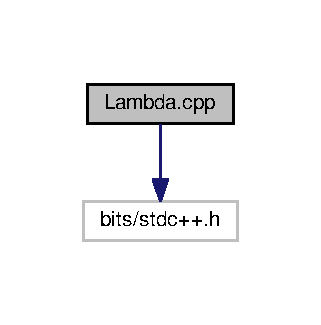
\includegraphics[width=154pt]{Lambda_8cpp__incl}
\end{center}
\end{figure}
\subsection*{Functions}
\begin{DoxyCompactItemize}
\item 
void \hyperlink{Lambda_8cpp_a6604e53b47269028db86484b041edbc1}{print\+Vector} (vector$<$ int $>$ v)
\item 
int \hyperlink{Lambda_8cpp_ae66f6b31b5ad750f1fe042a706a4e3d4}{main} ()
\end{DoxyCompactItemize}


\subsection{Function Documentation}
\index{Lambda.\+cpp@{Lambda.\+cpp}!main@{main}}
\index{main@{main}!Lambda.\+cpp@{Lambda.\+cpp}}
\subsubsection[{\texorpdfstring{main()}{main()}}]{\setlength{\rightskip}{0pt plus 5cm}int main (
\begin{DoxyParamCaption}
{}
\end{DoxyParamCaption}
)}\hypertarget{Lambda_8cpp_ae66f6b31b5ad750f1fe042a706a4e3d4}{}\label{Lambda_8cpp_ae66f6b31b5ad750f1fe042a706a4e3d4}

\begin{DoxyCode}
17 \{
18     vector<int> v \{4, 1, 3, 5, 2, 3, 1, 7\};
19 
20     \hyperlink{Lambda_8cpp_a6604e53b47269028db86484b041edbc1}{printVector}(v);
21 
22     \textcolor{comment}{// below snippet find first number greater than 4}
23     \textcolor{comment}{// find\_if searches for an element for which}
24     \textcolor{comment}{// function(third argument) returns true}
25     vector<int>:: iterator p = find\_if(v.begin(), v.end(), [](\textcolor{keywordtype}{int} i)
26     \{
27         \textcolor{keywordflow}{return} i > 4;
28     \});
29     cout << \textcolor{stringliteral}{"First number greater than 4 is : "} << *p << endl;
30 
31 
32     \textcolor{comment}{// function to sort vector, lambda expression is for sorting in}
33     \textcolor{comment}{// non-decreasing order Compiler can make out return type as}
34     \textcolor{comment}{// bool, but shown here just for explanation}
35     sort(v.begin(), v.end(), [](\textcolor{keyword}{const} \textcolor{keywordtype}{int}& a, \textcolor{keyword}{const} \textcolor{keywordtype}{int}& b) -> \textcolor{keywordtype}{bool}
36     \{
37         \textcolor{keywordflow}{return} a > b;
38     \});
39 
40     \hyperlink{Lambda_8cpp_a6604e53b47269028db86484b041edbc1}{printVector}(v);
41 
42     \textcolor{comment}{// function to count numbers greater than or equal to 5}
43     \textcolor{keywordtype}{int} count\_5 = count\_if(v.begin(), v.end(), [](\textcolor{keywordtype}{int} a)
44     \{
45         \textcolor{keywordflow}{return} (a >= 5);
46     \});
47     cout << \textcolor{stringliteral}{"The number of elements greater than or equal to 5 is : "}
48         << count\_5 << endl;
49 
50     \textcolor{comment}{// function for removing duplicate element (after sorting all}
51     \textcolor{comment}{// duplicate comes together)}
52     p = unique(v.begin(), v.end(), [](\textcolor{keywordtype}{int} a, \textcolor{keywordtype}{int} b)
53     \{
54         \textcolor{keywordflow}{return} a == b;
55     \});
56 
57     \textcolor{comment}{// resizing vector to make size equal to total different number}
58     v.resize(distance(v.begin(), p));
59     \hyperlink{Lambda_8cpp_a6604e53b47269028db86484b041edbc1}{printVector}(v);
60 
61     \textcolor{comment}{// accumulate function accumulate the container on the basis of}
62     \textcolor{comment}{// function provided as third argument}
63     \textcolor{keywordtype}{int} arr[] = \{1, 2, 3, 4, 5, 6, 7, 8, 9, 10\};
64     \textcolor{keywordtype}{int} f = accumulate(arr, arr + 10, 1, [](\textcolor{keywordtype}{int} i, \textcolor{keywordtype}{int} j)
65     \{
66         \textcolor{keywordflow}{return} i * j;
67     \});
68 
69     cout << \textcolor{stringliteral}{"Factorial of 10 is : "} << f << endl;
70 
71     \textcolor{comment}{// We can also access function by storing this into variable}
72     \textcolor{keyword}{auto} square = [](\textcolor{keywordtype}{int} i)
73     \{
74         \textcolor{keywordflow}{return} i * i;
75     \};
76 
77     cout << \textcolor{stringliteral}{"Square of 5 is : "} << square(5) << endl;
78 \}
\end{DoxyCode}


Here is the call graph for this function\+:
\nopagebreak
\begin{figure}[H]
\begin{center}
\leavevmode
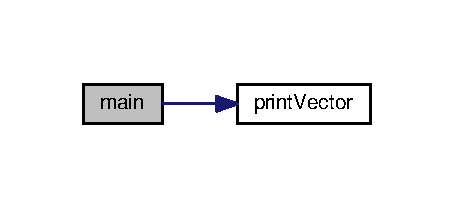
\includegraphics[width=218pt]{Lambda_8cpp_ae66f6b31b5ad750f1fe042a706a4e3d4_cgraph}
\end{center}
\end{figure}


\index{Lambda.\+cpp@{Lambda.\+cpp}!print\+Vector@{print\+Vector}}
\index{print\+Vector@{print\+Vector}!Lambda.\+cpp@{Lambda.\+cpp}}
\subsubsection[{\texorpdfstring{print\+Vector(vector$<$ int $>$ v)}{printVector(vector< int > v)}}]{\setlength{\rightskip}{0pt plus 5cm}void print\+Vector (
\begin{DoxyParamCaption}
\item[{vector$<$ int $>$}]{v}
\end{DoxyParamCaption}
)}\hypertarget{Lambda_8cpp_a6604e53b47269028db86484b041edbc1}{}\label{Lambda_8cpp_a6604e53b47269028db86484b041edbc1}

\begin{DoxyCode}
7 \{
8     \textcolor{comment}{// lambda expression to print vector}
9     for\_each(v.begin(), v.end(), [](\textcolor{keywordtype}{int} i)
10     \{
11         std::cout << i << \textcolor{stringliteral}{" "};
12     \});
13     cout << endl;
14 \}
\end{DoxyCode}

%--- End generated contents ---

% Index
\backmatter
\newpage
\phantomsection
\clearemptydoublepage
\addcontentsline{toc}{chapter}{Index}
\printindex

\end{document}
